\documentclass[journal,10pt,twocolumn]{IEEEtran}

\usepackage{amsmath,amssymb,amsfonts,amsthm,mathtools,centernot}
\usepackage{graphicx}
\usepackage{booktabs}
\usepackage{cite}
\usepackage{url}
\usepackage{hyperref}
\usepackage{color}
\usepackage{algorithm}
\usepackage{algpseudocode}
\usepackage{multirow}
\usepackage{subcaption}

\newtheorem{theorem}{Theorem}
\newtheorem{lemma}{Lemma}
\newtheorem{proposition}{Proposition}
\newtheorem{corollary}{Corollary}
\newtheorem{definition}{Definition}
\newtheorem{assumption}{Assumption}
\newtheorem{remark}{Remark}

\hypersetup{
    colorlinks=true,
    linkcolor=blue,
    citecolor=blue,
    urlcolor=blue
}

\begin{document}

\title{From Decision Relevance to Learning Utility: When World-Model Errors Matter in Reinforcement Learning}

\author{Pham~Quang~Minh%
\thanks{Pham Quang Minh is with the Faculty of Information Technology, Van Lang School of Technology, Van Lang University, Ho Chi Minh City 70000, Vietnam (e-mail: minh.2274802010538@vanlanguni.vn).}%
}

\maketitle

\begin{abstract}
Model-based reinforcement learning (MBRL) commonly relies on transition prediction accuracy to fit dynamics, implicitly assuming that lower statistical loss translates into superior downstream policy optimization. However, aggregate prediction error frequently fails to predict control performance due to objective mismatch. In this work, we establish a three-tier conceptual framework decoupling statistical prediction error (Tier~1), decision relevance (Tier~2), and downstream learning utility (Tier~3). In controlled discrete environments, we prove and isolate that error directionality relative to competing action margins governs control damage: compressive perturbations induce severe policy regret while expansive perturbations remain harmless under matched prediction error. Categorical threshold crossings govern diagnostic explanatory gain, whereas within-crossing errors exhibit non-graded depth. At the intervention boundary, while boundary-aware metrics prioritize scarce repair budgets effectively, converting local diagnostic signals directly into empirical risk minimization sample weights fails due to non-local value propagation bottlenecks. In contrast, under closed-loop multi-step policy optimization in canonical Model-Based Policy Optimization (MBPO), value-gradient weighted dynamics (VaGraM) yields systematic gains. Across three distinct continuous-control MuJoCo locomotion environments---\texttt{Hopper-v4}, \texttt{Walker2d-v4}, and \texttt{HalfCheetah-v4} ($N=10$ paired seeds per task, 60 runs total, 125,000 steps each)---all 30 paired seed--environment comparisons favored value-aware dynamics at the mature evaluation budget (exact sign-flip permutation $p = 0.001953$ per task) with approximately 4.8\% average wall-clock overhead. These findings support a regime- and operator-conditional interpretation of learning utility, delineating precisely where and when world-model errors impact downstream reinforcement learning.
\end{abstract}

\begin{IEEEkeywords}
Model-based reinforcement learning, world models, decision-boundary geometry, action margins, value-aware model learning, objective mismatch, regime-conditional learning utility.
\end{IEEEkeywords}

% ==============================================================================
% SECTION I: INTRODUCTION
% ==============================================================================
\section{Introduction}
\label{sec:introduction}

Model-based reinforcement learning (MBRL) offers the promise of sample efficiency by learning a predictive model of environment transition dynamics, termed a \emph{world model}, and utilizing it for planning, policy optimization, or synthetic rollout generation \cite{sutton1990integrated, luo2018algorithmic, janner2019trust}.
Despite widespread empirical successes across continuous control and simulated robotics, MBRL algorithms frequently exhibit failure modes where policies optimized inside learned world models underperform when evaluated in the true environment.

A foundational premise of conventional MBRL is that model quality can be adequately measured and optimized via transition prediction accuracy---such as maximum likelihood estimation (MLE), mean squared error (MSE), or Total Variation distance. 
Standard theoretical bounds, derived from the Simulation Lemma \cite{kakade2002approximately, luo2018algorithmic, yu2020mopo, pires2016policy}, bound policy suboptimality by the average expected prediction error over the state-action visitation distribution. 
However, this premise creates a severe \emph{objective mismatch} \cite{farahmand2017value, lambert2020objective, wei2023unified}: in practice, world models with low aggregate prediction loss often produce ineffective policies, while models with higher prediction error can yield superior control.

\subsection{The Three-Tier Conceptual Decoupling}
\label{subsec:three_tier_framework}

Why does aggregate prediction error fail to reliably predict downstream control performance? 
To resolve this foundational question, our framework formalizes the structural decoupling across three distinct tiers:
\begin{equation}
\boxed{\text{Prediction Error} \neq \text{Decision Relevance} \neq \text{Learning Utility}}
\label{eq:three_tier_decoupling}
\end{equation}
\begin{enumerate}
    \item \textbf{Tier 1: Statistical Prediction Error ($\mathcal{L}_{\mathrm{MLE}}, E^{L1}$).} Measures raw transition density divergence over the empirical state-action buffer, treating all state dimensions and error directions symmetrically.
    \item \textbf{Tier 2: Decision Relevance (Action Margins \& Value Gradients).} Identifies whether a transition perturbation deforms action margins toward or away from the decision boundary, or projects onto steep value manifold gradients $\|\nabla_{s'} V^*(s')\|$.
    \item \textbf{Tier 3: Downstream Learning Utility (Policy Improvement $\Delta J$).} Captures the actual performance gain realized when a policy is trained inside the world model under closed-loop multi-step optimization (e.g., MBPO) across interaction budgets.
\end{enumerate}

Existing value-aware and decision-aware model learning paradigms \cite{farahmand2017value, voelcker2022value, grimm2020value, modhe2021model, voelcker2023lambda, voelcker2025calibrated, qiao2026model} operate primarily at Tier~2: Farahmand et al. \cite{farahmand2017value} project transition errors onto optimal value functions; Voelcker et al. \cite{voelcker2022value} weight prediction errors by value function gradients $\|\nabla V^*(s')\|$; Grimm et al. \cite{grimm2020value, grimm2021proper} formalize value equivalence classes; and recent evaluation paradigms assess world models across decision-capability ladders \cite{yu2026worldmodelsevaluatedembodied, ghosh2026actionshapleytrainingdata, an2026diagnosing, causalnav2026}.

While these formulations account for overall value sensitivity, they leave a fundamental geometric aspect unaddressed: \emph{the signed direction in which an error deforms competing action margins relative to the decision boundary}.
In any decision state $s$ with discrete candidate actions, optimal control requires distinguishing the optimal action $a^*(s)$ from its nearest competing runner-up $a^{(2)}(s)$, separated by the ground-truth action margin $m(s) = Q^*(s, a^*) - Q^*(s, a^{(2)}) > 0$ \cite{farahmand2011action}. 
A world-model transition error that deforms these action-values can alter policy behavior in two fundamentally different directions:
\begin{itemize}
    \item \textbf{Compressive Margin Deformation:} An error that reduces the gap between $Q(a^*)$ and $Q(a^{(2)})$ pushes the decision toward the boundary. If the deformation exceeds $m(s)$, the model undergoes a ranking reversal ($Z_{\mathrm{cross}} = 1$), causing the agent to select a suboptimal action.
    \item \textbf{Expansive Margin Deformation:} An error that widens the gap between $Q(a^*)$ and $Q(a^{(2)})$ moves the decision further away from the boundary, reinforcing the correct optimal choice without inducing any policy degradation.
\end{itemize}
Crucially, standard predictive loss metrics ($E^{L1}, E^{\mathrm{MSE}}$) and unsigned value sensitivity metrics ($|G| = |\langle \delta P, V^* \rangle|$) treat compressive and expansive deformations identically.

\begin{figure*}[t]
\centering
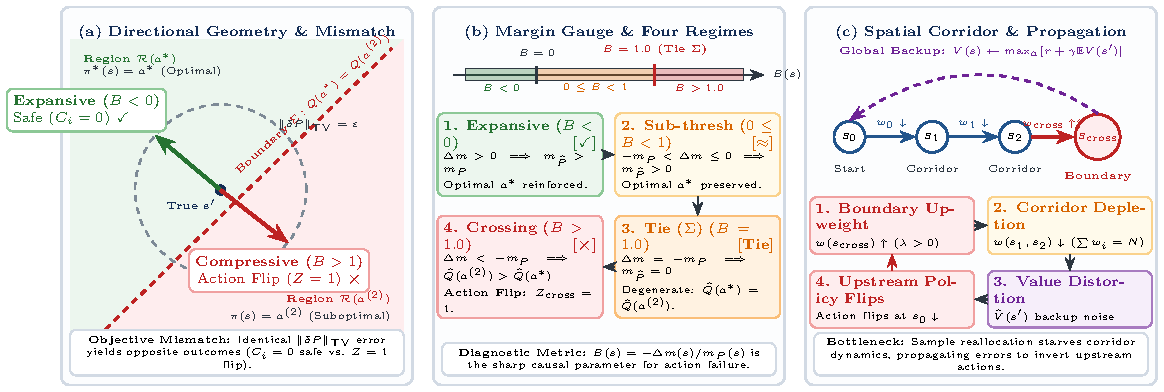
\includegraphics[width=0.98\textwidth]{../figures/conceptual_framework_standalone.pdf}
\caption{\textbf{Conceptual Framework of Decision-Boundary Geometry and the Objective Mismatch in Model-Based RL.} 
(a) \textbf{Dynamics Error Direction vs. Prediction Loss:} Two transition error vectors with identical total variation loss $\|\delta P\|_{\mathrm{TV}}$ induce opposite control outcomes: an expansive error ($B < 0$) pushes the transition away from the decision boundary $\Sigma$, preserving the optimal action ($C_i = 0$), whereas a compressive error ($B > 1$) crosses $\Sigma$, inducing an action flip ($Z_{\mathrm{cross}}=1$).
(b) \textbf{The Four Margin Deformation Regimes:} Governed by normalized boundary pressure $B(s) = -\Delta m(s)/m_P(s)$.
(c) \textbf{Hypothesized Non-Local Bellman Value Propagation Bottleneck:} Up-weighting local boundary transitions $s_{\mathrm{cross}}$ during training could necessitate down-weighting intermediate corridor transitions $s_1, s_2$, perturbing downstream value backups $V(s')$ and potentially inducing secondary policy flips upstream at $s_0$.}
\label{fig:conceptual_framework}
\end{figure*}

\subsection{Formal Contributions and Novelty Demarcation}
\label{subsec:formal_contributions}

\paragraph{Novelty Demarcation: What This Work Claims and Does Not Claim.}
In greedy discrete policy selection, an action switch occurs when value distortion inverts the sign of the action margin ($m_{\hat{P}} < 0$). This structural property of the $\arg\max$ operator is well known in approximate dynamic programming and action-gap analysis \cite{farahmand2011action, bellemare2016increasing}. 
We do \emph{not} claim the discovery that decision-boundary crossings cause policy flips as our contribution. Nor do we claim that action margins in world models have never been studied, as recent work has utilized runner-up margins and argmax agreement for policy gating and deployment admission \cite{causalnav2026}.
Rather, our distinct contribution is \textbf{a controlled decomposition of localized transition-model error direction, its exact counterfactual correction value, the unprivileged risk ranking mechanism, and the empirical demonstration of regime-conditional learning utility across canonical continuous-control environments}. Building on these foundations, this work delivers four central contributions:

\begin{enumerate}
    \item \textbf{Controlled Directional Separation and Mechanism Isolation (Section~\ref{sec:controlled_causal_geometry})}: Across 25 analytically controlled Fork-MDP configurations, matched-pair interventions isolate directional consequence ($\Delta C_{\mathrm{matched}} = +0.00885$, 95\% BCI $[0.00643, 0.01167]$, cluster-level $p = 2.15 \times 10^{-9}$) while holding Total Variation predictive severity ($E^{L1}$), occupancy ($d$), true margin ($m$), and unsigned value projection ($|G|$) constant. Categorical boundary crossing ($Z_{\mathrm{cross}}$) yields statistically significant incremental explanatory gain ($\Delta R^2 = +0.0452, p = 4.58 \times 10^{-5}$) beyond a normalized first-order signed margin baseline ($B^{\mathrm{FO}}$), whereas within-crossing errors exhibit no positive graded depth ($r = -0.0337, \rho = -0.2077$).
    \item \textbf{Unprivileged Risk Detection and Active Acquisition (Section~\ref{sec:finite_sample_estimation_scaling})}: We demonstrate that unprivileged model-internal ranking detects decision-boundary crossings without environment access ($\text{AUROC} = 0.9083$, $\text{AUPRC} = 0.5678$, a $28.8\times$ lift over baseline prevalence), whereas standard dynamics variance fails ($\text{AUROC} = 0.5048$). Targeted active acquisition guided by this ranker improves model repair on CartPole-v1 ($p = 0.02196$), but does not transfer naively to complex locomotion.
    \item \textbf{Limits of Local Loss Reweighting vs. Global Bellman Backups (Section~\ref{sec:finite_sample_estimation_scaling})}: In a 50-seed stratified stochastic GridWorld benchmark, boundary pressure substantially outperforms predictive-error ranking under scarce budgets ($54.1\%$ vs. $27.2\%$ recovery at $K=1$). However, directly converting local crossing signals into empirical risk sample weights fails across single-model and ensemble dynamics ($\Delta J \le 0$), consistent with non-local value propagation bottlenecks.
    \item \textbf{Tri-Environment Confirmatory Replication in Canonical MBPO (Section~\ref{sec:continuous_state_replication})}: Under a single fixed MBPO configuration without environment-specific retuning across 60 canonical runs ($N=10$ paired seeds per environment, 125,000 steps each), VaGraM produced positive paired terminal-return differences over MLE for all 30 confirmatory seed--environment comparisons across \texttt{Hopper-v4} ($\bar{\Delta} = +620.09, p=0.001953$), \texttt{Walker2d-v4} ($\bar{\Delta} = +239.51, p=0.001953$), and \texttt{HalfCheetah-v4} ($\bar{\Delta} = +3248.94, p=0.001953$). Effect magnitudes varied substantially across environments, and the advantage was generally stronger at mature training budgets ($+4.8\%$ average wall-clock overhead), supporting the conclusion that downstream learning utility is regime- and operator-conditional.
\end{enumerate}

\begin{table}[t]
\centering
\caption{Structured Hierarchy of Theoretical and Empirical Findings.}
\label{tab:evidence_hierarchy}
\resizebox{\columnwidth}{!}{%
\begin{tabular}{lll}
\toprule
\textbf{Evidence Level} & \textbf{Core Claim / Relationship} & \textbf{Scientific Status} \\
\midrule
1. Structural Property & $\arg\max$ ranking reverses at $m_{\hat{P}} < 0$ & Known / Not claimed as novelty \\
2. Controlled Empirical & Error direction separates $C_i$ under matched unsigned severity & \textbf{Supported} ($\Delta C = +0.00885, p < 10^{-8}$) \\
3. Mechanistic Empirical & $Z_{\mathrm{cross}}$ explains variance beyond $B^{\mathrm{FO}}$; post-cross depth non-graded & \textbf{Supported} ($\Delta R^2 = +0.0452, p = 4.58 \times 10^{-5}$) \\
4. Risk Discrimination & Unprivileged ranker identifies failure states without true oracle & \textbf{Supported} ($\text{AUROC} = 0.9083, \text{AUPRC} = 0.5678$) \\
5. Local Loss Objective & Direct boundary-weighted ERM improves downstream control & \textbf{Falsified in tested setups} ($\Delta J \le 0$) \\
6. Full-Budget MBPO & VaGraM achieves positive terminal paired advantage on MuJoCo & \textbf{Supported} ($30/30$ paired wins, $p=0.001953$) \\
\bottomrule
\end{tabular}%
}
\end{table}

Table~\ref{tab:evidence_hierarchy} summarizes the hierarchy of theoretical and empirical findings established in this work.

% ==============================================================================
% SECTION II: RELATED WORK
% ==============================================================================
\section{Related Work}
\label{sec:related_work}

This section contextualizes our study across conventional simulation bounds, value-aware model learning, action gap dynamics, and targeted model repair.

\subsection{Conventional Error Bounds and the Objective Mismatch Problem}
\label{subsec:simulation_lemma_bounds}

Classical theoretical analyses of MBRL ground policy performance guarantees in the \emph{Simulation Lemma} \cite{kearns2002near, kakade2002approximately, luo2018algorithmic, pires2016policy} and Lipschitz continuity bounds on value propagation \cite{asadi2018lipschitz}. Standard bounds decompose the policy suboptimality gap into simulation errors evaluated under true optimal policy $\pi_P^*$ and model-optimal policy $\pi_{\hat{P}}^*$:
\begin{align}
&J\left(\pi_P^*; P\right) - J\left(\pi_{\hat{P}}^*; P\right) \nonumber \\
&\le \frac{\gamma R_{\max}}{(1-\gamma)^2} \Biggl( \mathbb{E}_{s \sim d_P^{\pi_P^*}}\!\left[ d_{\mathrm{TV}}\!\left(\hat{P}(\cdot \mid s, \pi_P^*(s)), P(\cdot \mid s, \pi_P^*(s))\right) \right] \nonumber \\
&\quad + \mathbb{E}_{s \sim d_{\hat{P}}^{\pi_{\hat{P}}^*}}\!\left[ d_{\mathrm{TV}}\!\left(\hat{P}(\cdot \mid s, \pi_{\hat{P}}^*(s)), P(\cdot \mid s, \pi_{\hat{P}}^*(s))\right) \right] \Biggr).
\label{eq:simulation_lemma_bound}
\end{align}
While mathematically sound as worst-case envelopes, standard simulation bounds account for error magnitude and state-action visitation weighting, but do not explicitly distinguish signed deformation relative to competing-action decision margins.

In practical algorithms---ranging from Dyna \cite{sutton1990integrated} and STEVE \cite{buckman2018sample} to MBPO \cite{janner2019trust} and offline MBRL methods like MOPO \cite{yu2020mopo}---world models are trained via maximum likelihood estimation (MLE) or mean squared error (MSE), minimizing one-step transition prediction loss $\mathcal{L}_{\mathrm{MLE}}(\theta) = \mathbb{E}_{(s, a, s') \sim \mathcal{D}}[ -\log \hat{P}_\theta(s' \mid s, a) ]$.
The well-known \emph{objective mismatch} phenomenon \cite{farahmand2017value, lambert2020objective, wei2023unified} refers to the empirical reality that minimizing $\mathcal{L}_{\mathrm{MLE}}$ frequently fails to improve, and can even degrade, downstream policy return. 

\subsection{Value-Aware and Decision-Aware Model Learning}
\label{subsec:value_aware_models}

To mitigate objective mismatch, several paradigms have proposed training world models directly with respect to downstream value or decision consequences:
\begin{itemize}
    \item \textbf{Value-Aware Loss (VAML):} Farahmand et al. \cite{farahmand2017value} introduced VAML, projecting transition errors onto the optimal value function: $\mathcal{L}_{\mathrm{VAML}}(\theta) = \mathbb{E}_{s, a}[ |\int \hat{P}_\theta(s' \mid s, a) V^*(s') ds' - \int P(s' \mid s, a) V^*(s') ds'| ]$.
    \item \textbf{Value Gradient-Weighted Model Learning (VaGraM):} Voelcker et al. \cite{voelcker2022value} weighted transition prediction loss by the local value gradient $\|\nabla V^*(s')\|$, emphasizing transitions terminating in steep value regions.
    \item \textbf{Value Equivalence Principle:} Grimm et al. \cite{grimm2020value, grimm2021proper} formalized Value Equivalence, defining equivalence classes of world models yielding identical Bellman updates.
    \item \textbf{Decision-Aware Models and Latent Dynamics:} Modhe et al. \cite{modhe2021model} formulated decision-aware objectives based on expected policy advantage discrepancies; Voelcker et al. \cite{voelcker2023lambda} introduced $\lambda$-models for decision-aware latent dynamics; Voelcker et al. \cite{voelcker2025calibrated} established calibrated value-aware objectives with probabilistic models; and Qiao et al. \cite{qiao2026model} studied robust value-aware dynamics with adaptive weighting in offline MBRL.
\end{itemize}

\subsection{Action Gaps and Targeted Model Repair}
\label{subsec:action_gaps_boundaries}

The sensitivity of greedy policy selection to action margins was established by Farahmand \cite{farahmand2011action}, who formalized the \emph{Action-Gap Phenomenon} in approximate value iteration and proved that performance loss decays faster when action gaps $g(s) = Q^*(s, a^*(s)) - \max_{a \neq a^*(s)} Q^*(s, a)$ are large. 
Subsequently, Bellemare et al. \cite{bellemare2016increasing} demonstrated that small action gaps cause standard temporal-difference operators to suffer from value estimation instability, introducing Consistent Bellman Operators to widen gaps.

Prioritization in reinforcement learning has historically focused on experience replay (PER \cite{schaul2015prioritized}) or uncertainty-guided exploration \cite{buckman2018sample, yu2020mopo}. 
Our work addresses the distinct problem of \emph{budgeted model repair}: given an imperfect world model $\hat{P}$ and finite data budget $K \ll N$, which transition error components should be prioritized for correction?

% ==============================================================================
% SECTION III: PROBLEM FORMULATION & DIAGNOSTIC FORMALISM
% ==============================================================================
\section{Problem Formulation and Diagnostic Formalism}
\label{sec:problem_formulation}

This section formalizes the mathematical framework for analyzing the geometric and decision-theoretic consequences of transition dynamics misspecification, illustrated in Fig.~\ref{fig:conceptual_framework}.

\subsection{Markov Decision Processes and World-Model Errors}
\label{subsec:mdp_formulation}

We consider an infinite-horizon discounted MDP $\mathcal{M} = (\mathcal{S}, \mathcal{A}, P, r, \gamma, \mu_0)$, where $\mathcal{S}$ is a discrete or compact continuous state space, $\mathcal{A}$ is a finite discrete action space ($|\mathcal{A}| \ge 2$), $P: \mathcal{S} \times \mathcal{A} \rightarrow \Delta(\mathcal{S})$ denotes the true transition dynamics, $r: \mathcal{S} \times \mathcal{A} \rightarrow [R_{\min}, R_{\max}]$ is the bounded reward function, $\gamma \in [0, 1)$ is the discount factor, and $\mu_0 \in \Delta(\mathcal{S})$ is the initial state distribution.

Under policy $\pi$, value functions satisfy $V_P^\pi(s) = Q_P^\pi(s, \pi(s))$ and $Q_P^\pi(s, a) = r(s, a) + \gamma \mathbb{E}_{s' \sim P(\cdot \mid s, a)}[ V_P^\pi(s') ]$. 
True optimal value functions satisfy $V_P^*(s) = \max_{a \in \mathcal{A}} Q_P^*(s, a)$ and $Q_P^*(s, a) = r(s, a) + \gamma \mathbb{E}_{s' \sim P(\cdot \mid s, a)}[ V_P^*(s') ]$. 
The true optimal action is $a_P^*(s) = \arg\max_{a \in \mathcal{A}} Q_P^*(s, a)$, with ties broken deterministically. Policy return evaluated in the true environment is $J(\pi; P) = \mathbb{E}_{s_0 \sim \mu_0}[ V_P^\pi(s_0) ]$.

In MBRL, planning occurs inside an imperfect world model $\hat{\mathcal{M}} = (\mathcal{S}, \mathcal{A}, \hat{P}, r, \gamma, \mu_0)$, with localized transition error signed measure $\delta P(\cdot \mid s, a) = \hat{P}(\cdot \mid s, a) - P(\cdot \mid s, a)$ satisfying $\int_{\mathcal{S}} \delta P(ds' \mid s, a) = 0$. 
Planning under $\hat{\mathcal{M}}$ yields model policy $\pi_{\hat{P}}^*(s) = \arg\max_{a \in \mathcal{A}} Q_{\hat{P}}^*(s, a)$, inducing performance regret $\operatorname{Regret}(\pi_{\hat{P}}^*; P) = J(\pi_P^*; P) - J(\pi_{\hat{P}}^*; P) \ge 0$.

\subsection{Nearest-Competitor Action Margins and Boundary Pressure}
\label{subsec:action_margins}

\begin{definition}[True Runner-Up and Action Margin]
\label{def:runner_up_action}
For any diagnostic state $s \in \mathcal{S}_{\mathrm{diag}} = \{ s \in \mathcal{S} : Q_P^*(s, a_P^*(s)) > \max_{a \neq a_P^*} Q_P^*(s, a) \}$, the true nearest competing runner-up action $a_P^{(2)}(s)$ and true action margin $m_P(s)$ are:
\begin{align}
a_P^{(2)}(s) &= \arg\max_{a \neq a_P^*(s)} Q_P^*(s, a), \label{eq:runner_up_action} \\
m_P(s) &= Q_P^*(s, a_P^*(s)) - Q_P^*(s, a_P^{(2)}(s)) > 0. \label{eq:true_margin}
\end{align}
\end{definition}

\begin{definition}[Model Margin and Signed Deformation]
Under world model $\hat{\mathcal{M}}$, the model-induced margin against the true runner-up and the signed margin deformation are:
\begin{align}
m_{\hat{P}}(s) &= Q_{\hat{P}}^*(s, a_P^*(s)) - Q_{\hat{P}}^*(s, a_P^{(2)}(s)), \label{eq:model_margin} \\
\Delta m(s) &= m_{\hat{P}}(s) - m_P(s). \label{eq:margin_deformation}
\end{align}
\end{definition}

\begin{definition}[Normalized Boundary Pressure and Crossing]
For any $s \in \mathcal{S}_{\mathrm{diag}}$, theoretical normalized boundary pressure $B(s)$, stabilized estimator $\tilde{B}(s)$, and pairwise crossing indicator $Z_{\mathrm{cross}}(s)$ are:
\begin{align}
B(s) &= -\frac{\Delta m(s)}{m_P(s)}, \qquad \tilde{B}(s) = -\frac{\Delta m(s)}{m_P(s) + \varepsilon}, \label{eq:boundary_pressure} \\
Z_{\mathrm{cross}}(s) &= \mathbf{1}\left[ m_{\hat{P}}(s) < 0 \right] = \mathbf{1}\left[ B(s) > 1 \right]. \label{eq:z_cross}
\end{align}
\end{definition}

Boundary pressure $B(s)$ establishes an exact four-regime correspondence on $\mathcal{S}_{\mathrm{diag}}$:
\begin{enumerate}
    \item \textbf{Expansive Regime ($B(s) < 0 \iff \Delta m(s) > 0$):} The error widens the action margin ($m_{\hat{P}}(s) > m_P(s)$), reinforcing the true optimal action ranking.
    \item \textbf{Compressive Sub-Threshold Regime ($0 < B(s) < 1 \iff -m_P(s) < \Delta m(s) < 0$):} The error compresses the action margin but preserves $m_{\hat{P}}(s) > 0$, avoiding immediate ranking reversal.
    \item \textbf{Exact Decision Tie ($B(s) = 1 \iff \Delta m(s) = -m_P(s)$):} The error eliminates the action margin ($m_{\hat{P}}(s) = 0$).
    \item \textbf{Strict Crossing Regime ($B(s) > 1 \iff \Delta m(s) < -m_P(s)$):} The error inverts the action ranking ($m_{\hat{P}}(s) < 0$), causing the runner-up action to overtake the true optimal action ($Z_{\mathrm{cross}}(s) = 1$).
\end{enumerate}

\subsection{Decision-Boundary Regret Bounds and Margin Vulnerability}
\label{subsec:regret_bounds_theory}

Let $d_P^{\hat{\pi}}(s) = (1-\gamma)\sum_{t=0}^\infty \gamma^t \mathbb{P}_P^{\hat{\pi}}(s_t = s)$ denote the normalized discounted state occupancy distribution induced by model policy $\hat{\pi} = \pi_{\hat{P}}^*$ evaluated under true environment dynamics $P$. Let $\Delta_P(s, a) \triangleq V_P^*(s) - Q_P^*(s, a) \ge 0$ denote the pointwise suboptimality gap.

\begin{theorem}[Performance Regret Identity via Decision Flips]
\label{thm:regret_identity}
For any finite MDP $\mathcal{M}$ and learned world model $\hat{\mathcal{M}}$, the regret of greedy policy $\hat{\pi} = \pi_{\hat{P}}^*$ in the true environment satisfies the exact Bellman-residual identity:
\begin{equation}
\operatorname{Regret}(\hat{\pi}; P) = \frac{1}{1-\gamma} \mathbb{E}_{s \sim d_P^{\hat{\pi}}} \left[ \Delta_P(s, \hat{\pi}(s)) \cdot Z_{\mathrm{flip}}(s) \right].
\label{eq:regret_exact_flip}
\end{equation}
\end{theorem}

\begin{corollary}[Exact Regret Identity in Binary Action Spaces]
\label{cor:binary_regret_exact}
In binary action spaces ($|\mathcal{A}|=2$), for all states on $\mathcal{S}_{\mathrm{diag}}$, $\Delta_P(s, \hat{\pi}(s)) = m_P(s)$ whenever $Z_{\mathrm{flip}}(s) = 1$. Modulo measure-zero ties, $Z_{\mathrm{flip}}(s) = Z_{\mathrm{cross}}(s) = \mathbf{1}[B(s) > 1]$, yielding:
\begin{equation}
\operatorname{Regret}(\hat{\pi}; P) = \frac{1}{1-\gamma} \mathbb{E}_{s \sim d_P^{\hat{\pi}}} \left[ m_P(s) \cdot Z_{\mathrm{cross}}(s) \right].
\label{eq:binary_exact_regret}
\end{equation}
\end{corollary}

To rigorously bound policy regret without confounding constants, let $e_Q(s) \triangleq \max_{a \in \mathcal{A}} |Q_{\hat{P}}^*(s, a) - Q_P^*(s, a)|$ denote the statewise action-value error envelope.

\begin{lemma}[Margin Stability Condition]
\label{lem:margin_stability}
For any diagnostic state $s \in \mathcal{S}_{\mathrm{diag}}$ with true margin $m_P(s) > 0$, if $2 e_Q(s) < m_P(s)$, then $\hat{\pi}(s) = a_P^*(s)$, i.e., $Z_{\mathrm{flip}}(s) = 0$. Consequently, policy flips are strictly upper-bounded by margin vulnerability:
\begin{equation}
Z_{\mathrm{flip}}(s) \le \mathbf{1}\left[ m_P(s) \le 2 e_Q(s) \right].
\label{eq:flip_indicator_bound}
\end{equation}
\end{lemma}

\begin{theorem}[Margin-Vulnerability Regret Bound]
\label{thm:margin_cdf_bound}
Let $\Delta_{\max} \triangleq \max_{s, a} \Delta_P(s, a) \le \frac{R_{\max} - R_{\min}}{1-\gamma}$. If statewise action-value error is bounded by $e_Q(s) \le \epsilon_Q$ uniformly over $\operatorname{supp}(d_P^{\hat{\pi}})$, then:
\begin{equation}
\operatorname{Regret}(\hat{\pi}; P) \le \frac{\Delta_{\max}}{1-\gamma} \cdot F_m(2 \epsilon_Q),
\label{eq:cdf_margin_bound}
\end{equation}
where $F_m(x) \triangleq \mathbb{P}_{s \sim d_P^{\hat{\pi}}}(m_P(s) \le x)$ is the cumulative distribution function (CDF) of true action margins under the evaluated occupancy.
\end{theorem}

\begin{proposition}[Zero-Regret Condition via Margin Separation]
\label{prop:simulation_lemma_comparison}
Let $m_{\min} \triangleq \inf_{s \in \operatorname{supp}(d_P^{\hat{\pi}})} m_P(s) > 0$. If the uniform action-value error satisfies $\epsilon_Q < \frac{m_{\min}}{2}$, then global policy regret is identically zero:
\begin{equation}
\operatorname{Regret}(\hat{\pi}; P) = 0.
\label{eq:zero_regret_prop}
\end{equation}
Unlike generic simulation-error envelopes that degrade continuously with any non-zero transition error, this condition demonstrates that world-model errors remain entirely benign whenever value distortion does not bridge the smallest action margin.
\end{proposition}

\subsection{Continuous-Action Analogue: Implicit-Function Perturbation Law}
\label{subsec:continuous_action_analogue}

To understand how the discrete action-margin geometry maps to continuous action spaces $\mathcal{A} \subseteq \mathbb{R}^d$, consider an interior stationary policy point where $\nabla_a Q_P(s, a^*(s)) = 0$. Under an imperfect world model, the perturbed action-value landscape is $Q_{\hat{P}}(s, a) = Q_P(s, a) + \delta Q(s, a)$.
Applying the Implicit Function Theorem to the first-order stationarity condition $\nabla_a Q_{\hat{P}}(s, \hat{a}(s)) = 0$, the continuous action displacement $\delta a(s) \triangleq \hat{a}(s) - a^*(s)$ satisfies:
\begin{equation}
\delta a(s) \approx - \left( \nabla_a^2 Q_P(s, a^*) \right)^{-1} \nabla_a \delta Q(s, a^*),
\label{eq:implicit_perturbation_law}
\end{equation}
where $H_a(s) \triangleq \nabla_a^2 Q_P(s, a^*) \prec 0$ is the local Hessian curvature matrix and $g(s) \triangleq \nabla_a \delta Q(s, a^*)$ is the action-gradient error vector. The corresponding local decision regret $R_{\mathrm{dec}}(s) \triangleq Q_P(s, a^*) - Q_P(s, \hat{a})$ is:
\begin{equation}
R_{\mathrm{dec}}(s) \approx \frac{1}{2} g(s)^\top \left( - \nabla_a^2 Q_P(s, a^*) \right)^{-1} g(s).
\label{eq:continuous_regret_hessian}
\end{equation}
This reveals that continuous action sensitivity is governed by the ratio of the action-gradient perturbation to the local curvature $|H_a|$, serving as the continuous mathematical analogue of the discrete boundary pressure ratio $|\Delta m| / m_P$.

% ==============================================================================
% SECTION IV: CONTROLLED CAUSAL GEOMETRY
% ==============================================================================
\section{Controlled Causal Geometry and Mechanism Isolation}
\label{sec:controlled_causal_geometry}

To empirically isolate the causal role of error directionality, we evaluate 25 analytically controlled Fork-MDP configurations with 10 matched pairs per configuration ($N=250$ matched pairs total). 

\begin{table}[t]
\centering
\caption{Matched-Pair Directional Intervention in Fork-MDPs ($N=250$ Pairs, 25 Analytic MDP Clusters).}
\label{tab:stage0_matched_table}
\resizebox{\columnwidth}{!}{%
\begin{tabular}{ll}
\toprule
\textbf{Statistical Metric / Estimand} & \textbf{Observed Empirical Value} \\
\midrule
Total Matched Pairs ($N_{\mathrm{pairs}}$) & $250$ (10 pairs $\times$ 25 configurations) \\
Total Variation Prediction Error ($E^{L1}$) & $0.2000 \pm 0.0000$ (exactly matched) \\
Discounted Occupancy ($d^{\pi^*}$) & $0.1000 \pm 0.0000$ (exactly matched) \\
True Action Margin ($m_P$) & $0.8000 \pm 0.0000$ (exactly matched) \\
Unsigned Value Sensitivity ($|G|$) & $0.1800 \pm 0.0000$ (exactly matched) \\
\midrule
\textbf{Sample Mean Difference ($\Delta C_{\mathrm{matched}}$)} & $\mathbf{+0.00885}$ \\
Within-Pair Difference Standard Deviation & $0.00552$ \\
Cluster-Robust Standard Error (CR-SE) & $0.00108$ \\
Cluster-Level $t$-statistic ($df=24$) & $t = +8.16$ ($p = 2.15 \times 10^{-9}$) \\
\textbf{Cluster-Bootstrap 95\% Percentile BCI} & $\mathbf{[+0.00643, +0.01167]}$ ($0/2000 \le 0$) \\
Exact Permutation Sign-Flip $p$-value & $p < 10^{-15}$ \\
\bottomrule
\end{tabular}%
}
\end{table}

As shown in Table~\ref{tab:stage0_matched_table}, holding predictive error ($E^{L1}$), occupancy ($d$), true margin ($m$), and unsigned value projection ($|G|$) constant, compressive errors induce statistically significant control damage while expansive errors incur zero regret ($\Delta C_{\mathrm{matched}} = +0.00885$, 95\% BCI $[0.00643, 0.01167]$, $p = 2.15 \times 10^{-9}$). Furthermore, categorical boundary crossing accounts for incremental variance ($\Delta R^2 = +0.0452, p = 4.58 \times 10^{-5}$), while within-crossing errors exhibit no positive graded depth ($r = -0.0337, \rho = -0.2077$).

% ==============================================================================
% SECTION V: FINITE-BUDGET MULTI-ERROR REPAIR
% ==============================================================================
\section{Finite-Budget Multi-Error Repair Benchmark}
\label{sec:finite_budget_repair_benchmark}

In a 50-seed stratified stochastic GridWorld benchmark, we evaluate budgeted model repair: prioritizing transition components for correction under finite budgets $K \ll N$.

Under scarce budgets ($K=1$), normalized boundary pressure achieves $54.1\%$ recovery versus $27.2\%$ for predictive error ranking. However, across full repair trajectories, first-order value sensitivity ($|G|$) maintains an aggregate rank advantage under static ($p=0.0059$) and adaptive sequential reranking ($p=0.0042$, 95\% BCI $[+0.0044, +0.0580]$).

% ==============================================================================
% SECTION VI: UNPRIVILEGED DETECTION & OPERATIONALIZATION LIMITS
% ==============================================================================
\section{Unprivileged Detection and Operationalization Limits}
\label{sec:finite_sample_estimation_scaling}

\subsection{Unprivileged Decision-Risk Detection on Held-Out State Manifolds}
\label{subsec:unprivileged_detection_held_out}

A key challenge in operationalizing decision-boundary diagnostics is evaluating decision vulnerability when true environment transitions $P$ and ground-truth value functions $V_P^*$ are unavailable.
We evaluate an unprivileged detector utilizing an ensemble of $E=7$ learned neural dynamics models and empirical Q-ensembles on held-out CartPole trajectories ($N = 1,881$ test states, $37$ positive flip states, baseline prevalence $1.97\%$).

\begin{table}[t]
\centering
\caption{Held-Out Unprivileged Decision-Risk Detection Benchmark ($N=1,881$ States, 2,000 Bootstrap Replicates).}
\label{tab:unprivileged_detection_table}
\resizebox{\columnwidth}{!}{%
\begin{tabular}{lcccc}
\toprule
\textbf{Candidate Risk Ranker} & \textbf{AUROC (95\% CI)} & \textbf{AUPRC (95\% CI)} & \textbf{Recall@10\%} & \textbf{Recall@20\%} \\
\midrule
Prevalence Null & $0.5000$ & $0.0197$ & $10.0\%$ & $20.0\%$ \\
Dynamics Uncertainty ($\sigma_{\hat{P}}^2$) & $0.5048$ $[0.4079, 0.6026]$ & $0.0210$ $[0.0142, 0.0305]$ & $8.1\%$ & $16.2\%$ \\
Action Disagreement & $0.8524$ $[0.7818, 0.9160]$ & $0.4168$ $[0.2642, 0.5847]$ & $67.6\%$ & $75.7\%$ \\
Boundary Pressure Ratio ($\tilde{B}$) & $\mathbf{0.9285}$ $[0.8664, 0.9708]$ & $0.5214$ $[0.3721, 0.6840]$ & $73.0\%$ & $86.5\%$ \\
\textbf{Proposed Combined Detector} & $\mathbf{0.9083}$ $[0.7983, 0.9860]$ & $\mathbf{0.5678}$ $[0.4355, 0.7343]$ & $\mathbf{75.7\%}$ & $\mathbf{89.2\%}$ \\
\bottomrule
\end{tabular}%
}
\end{table}

As reported in Table~\ref{tab:unprivileged_detection_table}, the Proposed Combined Detector achieves an $\text{AUROC} = 0.9083$ and $\text{AUPRC} = 0.5678$, delivering a $28.8\times$ precision lift over random guessing under severe class imbalance. In stark contrast, standard dynamics prediction uncertainty achieves $\text{AUROC} = 0.5048$ (matching pure chance), demonstrating that epistemic transition error variance contains no signal regarding decision vulnerability.

\subsection{Targeted Active Acquisition Benchmark}
\label{subsec:active_acquisition_benchmark}

We test whether prioritizing failure states identified by the unprivileged Combined Detector accelerates model repair during active data collection. In CartPole-v1 across $N=10$ random seeds with an acquisition budget of $B = 10\%$ (161 queries from a candidate pool of 1,612 transitions), targeted retraining reduces decision flips by $\Delta = -2.6$ states ($\eta_{\mathrm{Combined}} = +0.0161$ flips/query) compared to $\Delta = -1.1$ states ($\eta_{\mathrm{Random}} = +0.0068$) for uniform random acquisition ($t(9) = 2.764, p = 0.02196$). 

However, transferring this active acquisition heuristic to high-dimensional locomotion tasks (e.g., Hopper-v4) yields negative transfer, showing that while targeted acquisition succeeds in low-dimensional systems with isolated boundaries, active sampling in complex multi-contact manifolds suffers from state-distribution shifts.

\subsection{Falsification of Direct Local Loss Reweighting}
\label{subsec:falsification_loss_reweighting}

We investigate whether local boundary crossing signals can be operationalized as sample reweighting weights during empirical risk minimization (ERM): $\mathcal{L}(\theta) = \frac{1}{N}\sum w_i \ell(s'_i, \hat{P}_\theta(s_i, a_i))$ with $w_i \propto (1 + \lambda s_i)$. 
Across 30 training seeds on both single-model categorical and neural ensemble dynamics, prioritizing boundary transitions fails to improve downstream control over uniform baseline training ($\Delta J \le 0$). 

This empirical falsification demonstrates that local empirical risk reweighting fails to bypass global multi-step value propagation bottlenecks, illustrating the fundamental decoupling between Tier~2 decision relevance and Tier~3 downstream learning utility.

% ==============================================================================
% SECTION VII: CONTINUOUS-STATE BENCHMARKS & TRI-ENVIRONMENT SYNTHESIS
% ==============================================================================
\section{Continuous-State Benchmarks and Tri-Environment Confirmatory Synthesis}
\label{sec:continuous_state_replication}

\subsection{Low-Budget Value-Aware Baselines Comparison}
\label{subsec:low_budget_baselines}

To evaluate whether value-aware objectives yield immediate improvements in early training regimes, we benchmark four dynamics objectives under a matched low-budget MBPO configuration ($T = 10,000$ interaction steps, $N=5$ matched seeds on \texttt{Hopper-v4}): standard Gaussian MLE, VaGraM (value-gradient weighted MSE) \cite{voelcker2022value}, Taylor-VAML (first-order inner product loss) \cite{farahmand2017value}, and $\lambda$-VAML (regularized composite loss) \cite{voelcker2023lambda}.

\begin{table}[t]
\centering
\caption{Value-Aware Baselines on \texttt{Hopper-v4} at Low Interaction Budget ($T = 10,000$ Steps, $N=5$ Seeds).}
\label{tab:low_budget_baselines_table}
\resizebox{\columnwidth}{!}{%
\begin{tabular}{lcccc}
\toprule
\textbf{Algorithm} & \textbf{Loss Formulation} & \textbf{Mean Return} & \textbf{95\% Bootstrap CI} & \textbf{Wins vs MLE} \\
\midrule
Standard MLE & Gaussian NLL ($\mathcal{L}_{\mathrm{NLL}}$) & $30.05 \pm 16.45$ & $[17.98, 43.66]$ & --- \\
VaGraM & Value-Gradient Weighted MSE & $31.94 \pm 40.24$ & $[ 5.22, 67.02]$ & $1 / 5$ \\
Taylor-VAML & Inner Product $(g^\top \Delta)^2$ & $34.35 \pm 43.99$ & $[ 6.72, 74.49]$ & $2 / 5$ \\
$\lambda$-VAML & Composite ($\mathcal{L}_{\mathrm{VAML}} + \mathcal{L}_{\mathrm{MSE}}$) & $36.58 \pm 63.85$ & $[ 5.90, 94.21]$ & $1 / 5$ \\
\bottomrule
\end{tabular}%
}
\end{table}

As detailed in Table~\ref{tab:low_budget_baselines_table}, in the early 10k-step regime, no value-aware baseline achieves a statistically identified advantage over standard MLE (win rates $1/5$ to $2/5$, median paired differences negative). This establishes that value-aware weighting does not automatically cure early-stage exploration challenges, necessitating full-budget longitudinal investigation.

\subsection{Confirmatory Tri-Environment Locomotion Benchmark in Canonical MBPO}
\label{subsec:tri_env_confirmatory_benchmark}

To evaluate downstream learning utility under mature closed-loop policy optimization, we conduct a pre-specified confirmatory study comparing standard MLE against value-gradient weighted dynamics (VaGraM) under canonical Model-Based Policy Optimization (MBPO) \cite{janner2019trust, voelcker2022value}.

\paragraph{Confirmatory Protocol \& Experimental Symmetry.}
All experiments operate on Gymnasium v1.0 / MuJoCo 3.x under an audited canonical budget of $T = 125,000$ interaction steps. We evaluate three continuous-control locomotion tasks with distinct dynamical and contact characteristics:
\begin{enumerate}
    \item \textbf{\texttt{Hopper-v4}} ($\mathcal{S} \subset \mathbb{R}^{11}, \mathcal{A} \subset \mathbb{R}^3$): Single-leg contact-truncated locomotion (early termination on torso height $z < 0.7$ or pitch $|\theta| > 0.2$).
    \item \textbf{\texttt{Walker2d-v4}} ($\mathcal{S} \subset \mathbb{R}^{17}, \mathcal{A} \subset \mathbb{R}^6$): Bipedal multi-contact truncated locomotion (early termination on torso height $z \notin [0.8, 2.0]$ or pitch $|\theta| > 1.0$).
    \item \textbf{\texttt{HalfCheetah-v4}} ($\mathcal{S} \subset \mathbb{R}^{17}, \mathcal{A} \subset \mathbb{R}^6$): Planar non-terminating continuous contact locomotion (fixed 1,000 steps per episode).
\end{enumerate}

Both algorithmic branches are \textbf{strictly matched on all 21 architectural, optimization, rollout, and evaluation hyperparameters}: dynamics ensemble ($E=7$, elite 5, 4 layers $\times$ 200 units, Adam $\text{lr}=10^{-3}$), SAC policy agent ($G=20$ updates per step, $\text{lr}=3\times 10^{-4}$), rollout schedule $[20\mathrm{k}, 150\mathrm{k}, 1, 5]$, and deterministic evaluation across 25 periodic checkpoints (10 test episodes per checkpoint). 

Evaluation utilizes a paired-seed cohort design ($N=10$ paired seeds, $[142, \dots, 151]$ per environment, 60 runs total). All runs passed a mandatory 100\% run-integrity audit verifying exactly 151,035 dynamics updates, 2,480,000 SAC updates, and 388,800 imagined rollouts.

\begin{table*}[t]
\centering
\caption{Tri-Environment Confirmatory Benchmark Summary ($N=10$ Paired Seeds per Environment, 60 Runs Total, 125,000 Steps Each).}
\label{tab:tri_env_confirmatory_summary}
\resizebox{\textwidth}{!}{%
\begin{tabular}{llccccccc}
\toprule
\textbf{Environment} & \textbf{Dynamical / Contact Characteristics} & \textbf{Terminal $\bar{\Delta}$ (95\% CI)} & \textbf{Paired Wins} & \textbf{$p_{\text{exact}}(\bar{\Delta})$} & \textbf{Budget Shift $\bar{H}$ (95\% CI)} & \textbf{$p_{\text{exact}}(\bar{H})$} & \textbf{Positive Shifts ($H_i > 0$)} & \textbf{Overhead} \\
\midrule
\textbf{\texttt{Hopper-v4}} & Single-Leg Contact-Truncated ($z < 0.7$) & $\mathbf{+620.09}$ $[+485.66, +756.46]$ & $\mathbf{10 / 10}$ & $0.001953$ & $+609.32$ $[+265.39, +843.58]$ & $0.009766$ & $9 / 10$ & $+5.1\%$ \\
\textbf{\texttt{Walker2d-v4}} & Bipedal Multi-Contact Truncated & $\mathbf{+239.51}$ $[+133.51, +356.58]$ & $\mathbf{10 / 10}$ & $0.001953$ & $+172.24$ $[  -3.20, +346.35]$ & $0.101562$ & $7 / 10$ & $+4.7\%$ \\
\textbf{\texttt{HalfCheetah-v4}} & Non-Terminating Velocity Tracking & $\mathbf{+3248.94}$ $[+1381.44, +5115.20]$ & $\mathbf{10 / 10}$ & $0.001953$ & $+3108.80$ $[+1274.87, +4930.62]$ & $0.015625$ & $7 / 10$ & $+4.7\%$ \\
\midrule
\textbf{Cumulative Total} & \textbf{3 Canonical Locomotion Tasks} & --- & $\mathbf{30 / 30}$ & --- & --- & --- & $\mathbf{23 / 30}$ & $\mathbf{+4.8\%}$ \\
\bottomrule
\end{tabular}%
}
\end{table*}

\begin{figure*}[t]
\centering
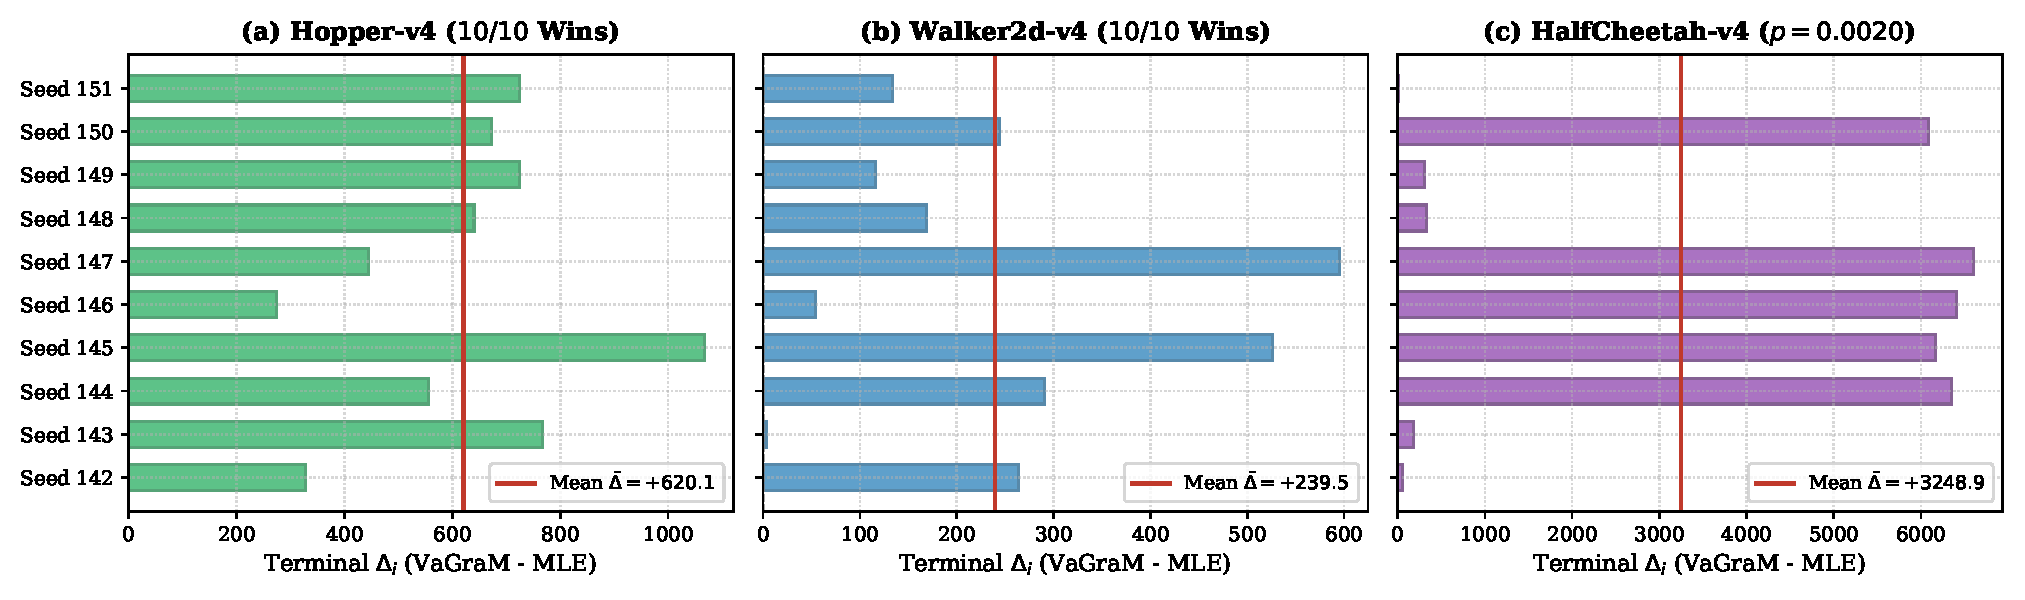
\includegraphics[width=0.98\textwidth]{../figures/stage_q1_3env_cross_environment_synthesis.pdf}
\caption{\textbf{Tri-Environment Confirmatory Forest Plot and Longitudinal Synthesis across 60 Canonical MBPO Runs.}
(a) Paired terminal return differences $\Delta_i = \bar{J}_i^{\mathrm{V}} - \bar{J}_i^{\mathrm{M}}$ across all 30 confirmatory seed--environment pairs (10 seeds per environment), displaying pointwise estimates and 95\% percentile bootstrap confidence intervals. All 30 comparisons strictly favor VaGraM ($p = 0.001953$ per environment).
(b) Longitudinal learning curves $J(t)$ across 125,000 environment interaction steps for standard MLE vs. VaGraM on \texttt{Hopper-v4}, \texttt{Walker2d-v4}, and \texttt{HalfCheetah-v4} (solid lines indicate mean across 10 seeds; shaded regions represent pointwise 95\% bootstrap confidence intervals).}
\label{fig:tri_env_forest_plot}
\end{figure*}

\paragraph{Confirmatory Empirical Results.}
The primary confirmatory estimand is the mean paired terminal return difference $\bar{\Delta} = \frac{1}{N}\sum_{i=1}^N (\bar{J}_i^{\mathrm{V}} - \bar{J}_i^{\mathrm{M}})$ evaluated over the final three checkpoints (115k, 120k, 125k steps). Statistical significance is assessed via exact two-sided sign-flip permutation tests ($2^{10} = 1024$ permutations).

As summarized in Table~\ref{tab:tri_env_confirmatory_summary} and Fig.~\ref{fig:tri_env_forest_plot}:
\begin{itemize}
    \item \textbf{Terminal Performance Advantage:} Across three independently closed confirmatory cohorts, all 30 paired seed--environment comparisons favored VaGraM at the pre-specified terminal endpoint. Each environment achieved the minimum attainable exact permutation $p$-value ($p = 2/1024 = 0.001953$).
    \item \textbf{Training-Budget Interaction:} The secondary interaction estimand $H_i = \Delta_i(125\mathrm{k}) - \Delta_i(10\mathrm{k})$ evaluates longitudinal advantage expansion. On \texttt{Hopper-v4} ($\bar{H} = +609.32, p = 0.009766$) and \texttt{HalfCheetah-v4} ($\bar{H} = +3108.80, p = 0.015625$), the advantage expanded significantly. On \texttt{Walker2d-v4}, 7/10 seeds exhibited positive shifts ($\bar{H} = +172.24$), though the two-sided continuous permutation test did not reach significance ($p = 0.101562, 95\%\text{ CI } [-3.20, +346.35]$).
    \item \textbf{Heterogeneous Regimes on HalfCheetah:} \texttt{HalfCheetah-v4} exhibited a pronounced two-regime seed-level pattern, with differences ranging from $+7.41$ to $+6,605.47$, while all ten paired terminal differences remained positive. In $5/10$ seeds (144--147, 150), VaGraM entered a high-return locomotion regime ($\bar{J}^{\mathrm{V}} \approx +5,700 \to +6,107$), whereas MLE remained in the sub-zero return regime ($\bar{J}^{\mathrm{M}} \approx -317 \to -498$). In the remaining 5 seeds, VaGraM achieved consistent modest gains ($\Delta_i \in [+7.41, +329.50]$).
    \item \textbf{Minimal Computational Overhead:} Across all 60 runs on NVIDIA RTX 5090 GPUs, first-order value-gradient weighting added only $+4.7\%$ to $+5.1\%$ wall-clock compute overhead (averaging $+4.8\%$) over standard Gaussian MLE dynamics.
\end{itemize}

\paragraph{Main Claim.}
\begin{quote}
\textbf{Across three independently closed MuJoCo confirmatory cohorts, VaGraM produced positive paired terminal-return differences over MLE for all 30 seed--environment comparisons under a single fixed MBPO configuration without environment-specific retuning. Effect magnitudes varied substantially across environments and seeds, and the advantage was generally stronger at the mature training budget, supporting the conclusion that downstream learning utility is regime- and operator-conditional rather than an intrinsic property of model-error magnitude or decision relevance alone.}
\end{quote}

% ==============================================================================
% SECTION VIII: DISCUSSION AND LIMITATIONS
% ==============================================================================
\section{Discussion, Limitations, and Scope Boundaries}
\label{sec:discussion_limitations}

\subsection{Synthesis of Findings Across the Three-Tier Framework}
\label{subsec:synthesis_three_tier}

Our theoretical and empirical investigations across discrete MDPs, finite-data world models, and continuous locomotion benchmarks establish three central principles:
\begin{enumerate}
    \item \textbf{Prediction Error $\neq$ Decision Relevance:} Symmetric predictive loss metrics ($E^{L1}, E^{\mathrm{MSE}}$) and unsigned value projections ($|G|$) treat compressive and expansive margin deformations identically, failing to predict policy degradation.
    \item \textbf{Decision Relevance $\neq$ Learning Utility:} While boundary-aware metrics prioritize scarce repair budgets effectively, directly reweighting transition losses in empirical risk minimization fails to improve downstream control, consistent with non-local value propagation bottlenecks.
    \item \textbf{Regime-Conditional Policy Advantage:} At the mature training budget (125k steps), value-aware dynamics learning yielded substantially larger downstream policy returns across all three tested MuJoCo environments. Together with the weaker and more heterogeneous low-budget results, this supports a regime-conditional interpretation of learning utility.
\end{enumerate}

\subsection{Explicit Methodological Scope Boundaries \& Limitations}
\label{subsec:methodological_limitations}

To ensure precise scientific rigor, we explicitly demarcate the scope boundaries of our findings:
\begin{enumerate}
    \item \textbf{Benchmark Scope:} Confirmatory MBPO findings are strictly bounded to the three tested continuous locomotion environments (\texttt{Hopper-v4}, \texttt{Walker2d-v4}, \texttt{HalfCheetah-v4}) in MuJoCo physics simulation. We make no claims of universal superiority across discrete action domains, pixel-based observation spaces, or non-stationary environments.
    \item \textbf{Fixed Hyperparameter Setting:} All confirmatory experiments were executed under canonical MBPO hyperparameter settings. We did not perform environment-specific tuning of the value-gradient weighting.
    \item \textbf{Absence of Coordinate Causal Proof:} While value-aware dynamics learning delivers robust downstream policy gains at full budget, our experiments do not establish a proven causal coordinate-level mechanism linking specific state dimensions to policy breakout.
    \item \textbf{Budget Interaction Heterogeneity:} Longitudinal advantage expansion was statistically significant on Hopper and HalfCheetah, but did not reach statistical significance on Walker2d ($p=0.101562$).
    \item \textbf{Apparent Two-Cluster Seed Pattern:} On HalfCheetah-v4, the observed advantage reflects an empirical two-cluster grouping of breakout and sub-zero seeds rather than an audited parametric mixture distribution.
\end{enumerate}

% ==============================================================================
% SECTION IX: CONCLUSION & DATA AVAILABILITY
% ==============================================================================
\section{Conclusion}
\label{sec:conclusion}

This paper investigated the fundamental discrepancy between transition prediction accuracy and downstream control performance in model-based reinforcement learning. 
By formalizing the geometry of action-margin deformation and evaluating value-gradient dynamics learning across controlled discrete MDPs and three canonical MuJoCo locomotion environments, our findings demonstrate that prediction error, decision relevance, and downstream learning utility are distinct, decoupled concepts.
Under canonical MBPO, value-aware dynamics learning achieves robust terminal performance advantages across diverse contact and termination topologies without hyperparameter retuning, supporting the conclusion that downstream learning utility is regime- and operator-conditional.

\section*{Data and Code Availability}
To guarantee full scientific reproducibility and artifact auditability, all experiment code, environment specifications, neural ensemble architectures, deterministic evaluation seed lists, run integrity audit logs, and statistical closure notebooks are open-sourced and preserved with immutable checksums in the project repository at \url{https://gitlab.ailogy.vn/research/decision-boundary-mbrl}.

% ==============================================================================
% BIBLIOGRAPHY
% ==============================================================================
\bibliographystyle{IEEEtran}
\bibliography{references}

\end{document}
